
\section{Experiments}

\begin{figure*}[t!]
    \centering
    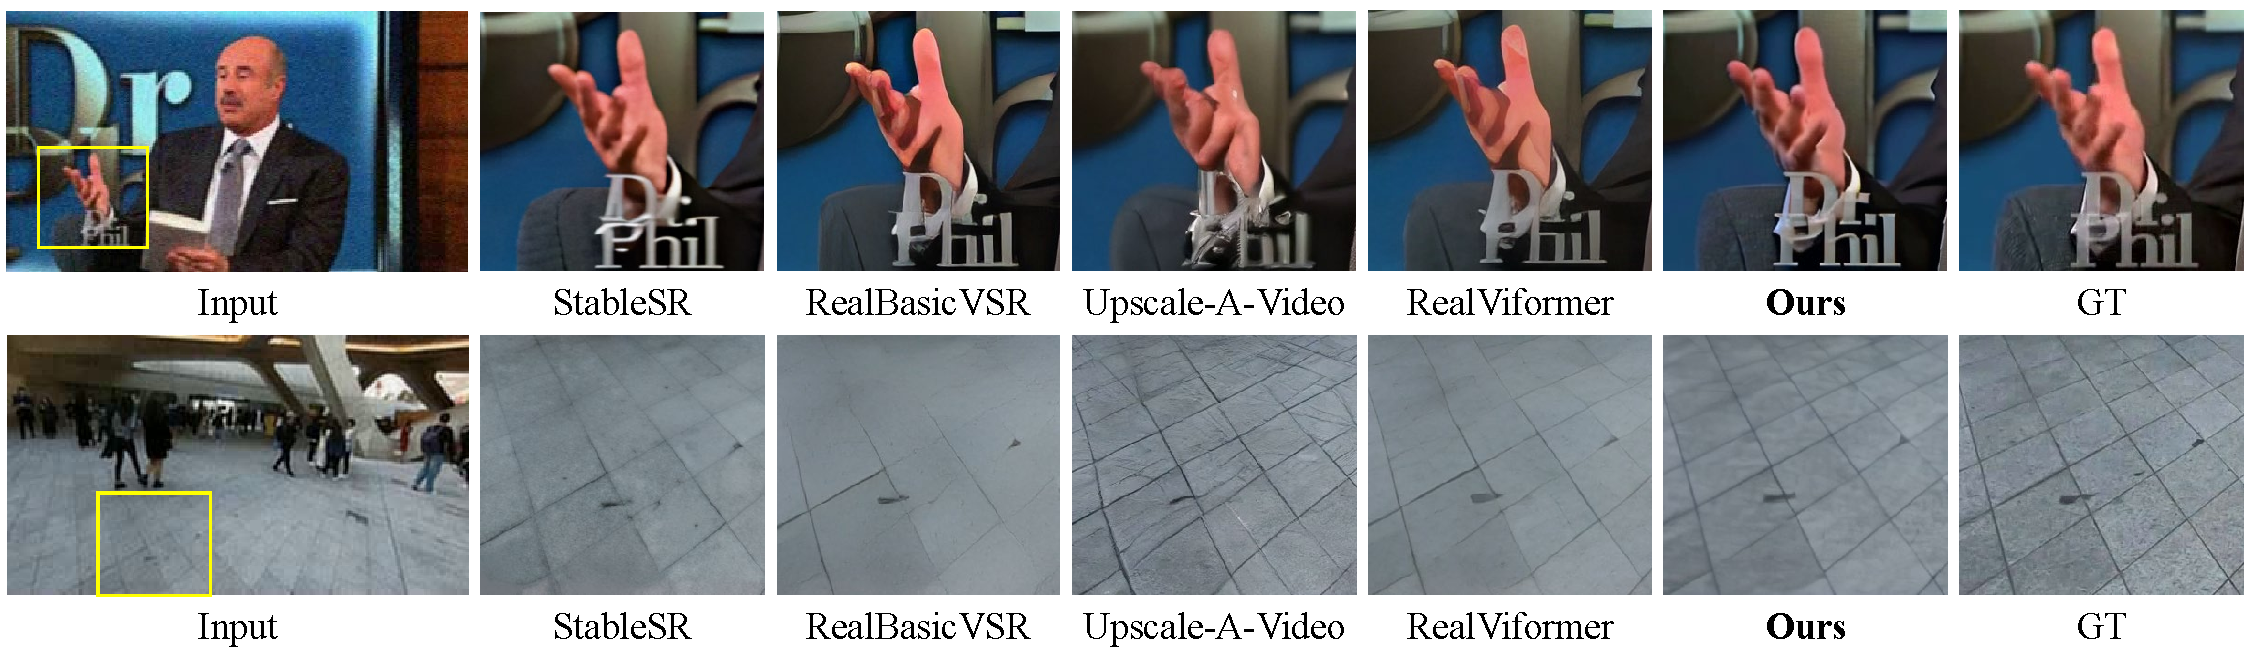
\includegraphics[width=1\linewidth]{figure/qualitive1.pdf}
    \caption{Qualitative comparisons on synthetic LR videos from OpenVid30 and REDS30\cite{nah2019ntire}. \textbf{(Zoom-in for best view)}}
    \label{fig:qualitive1}
\end{figure*}

\begin{figure*}[t!]
    \centering
    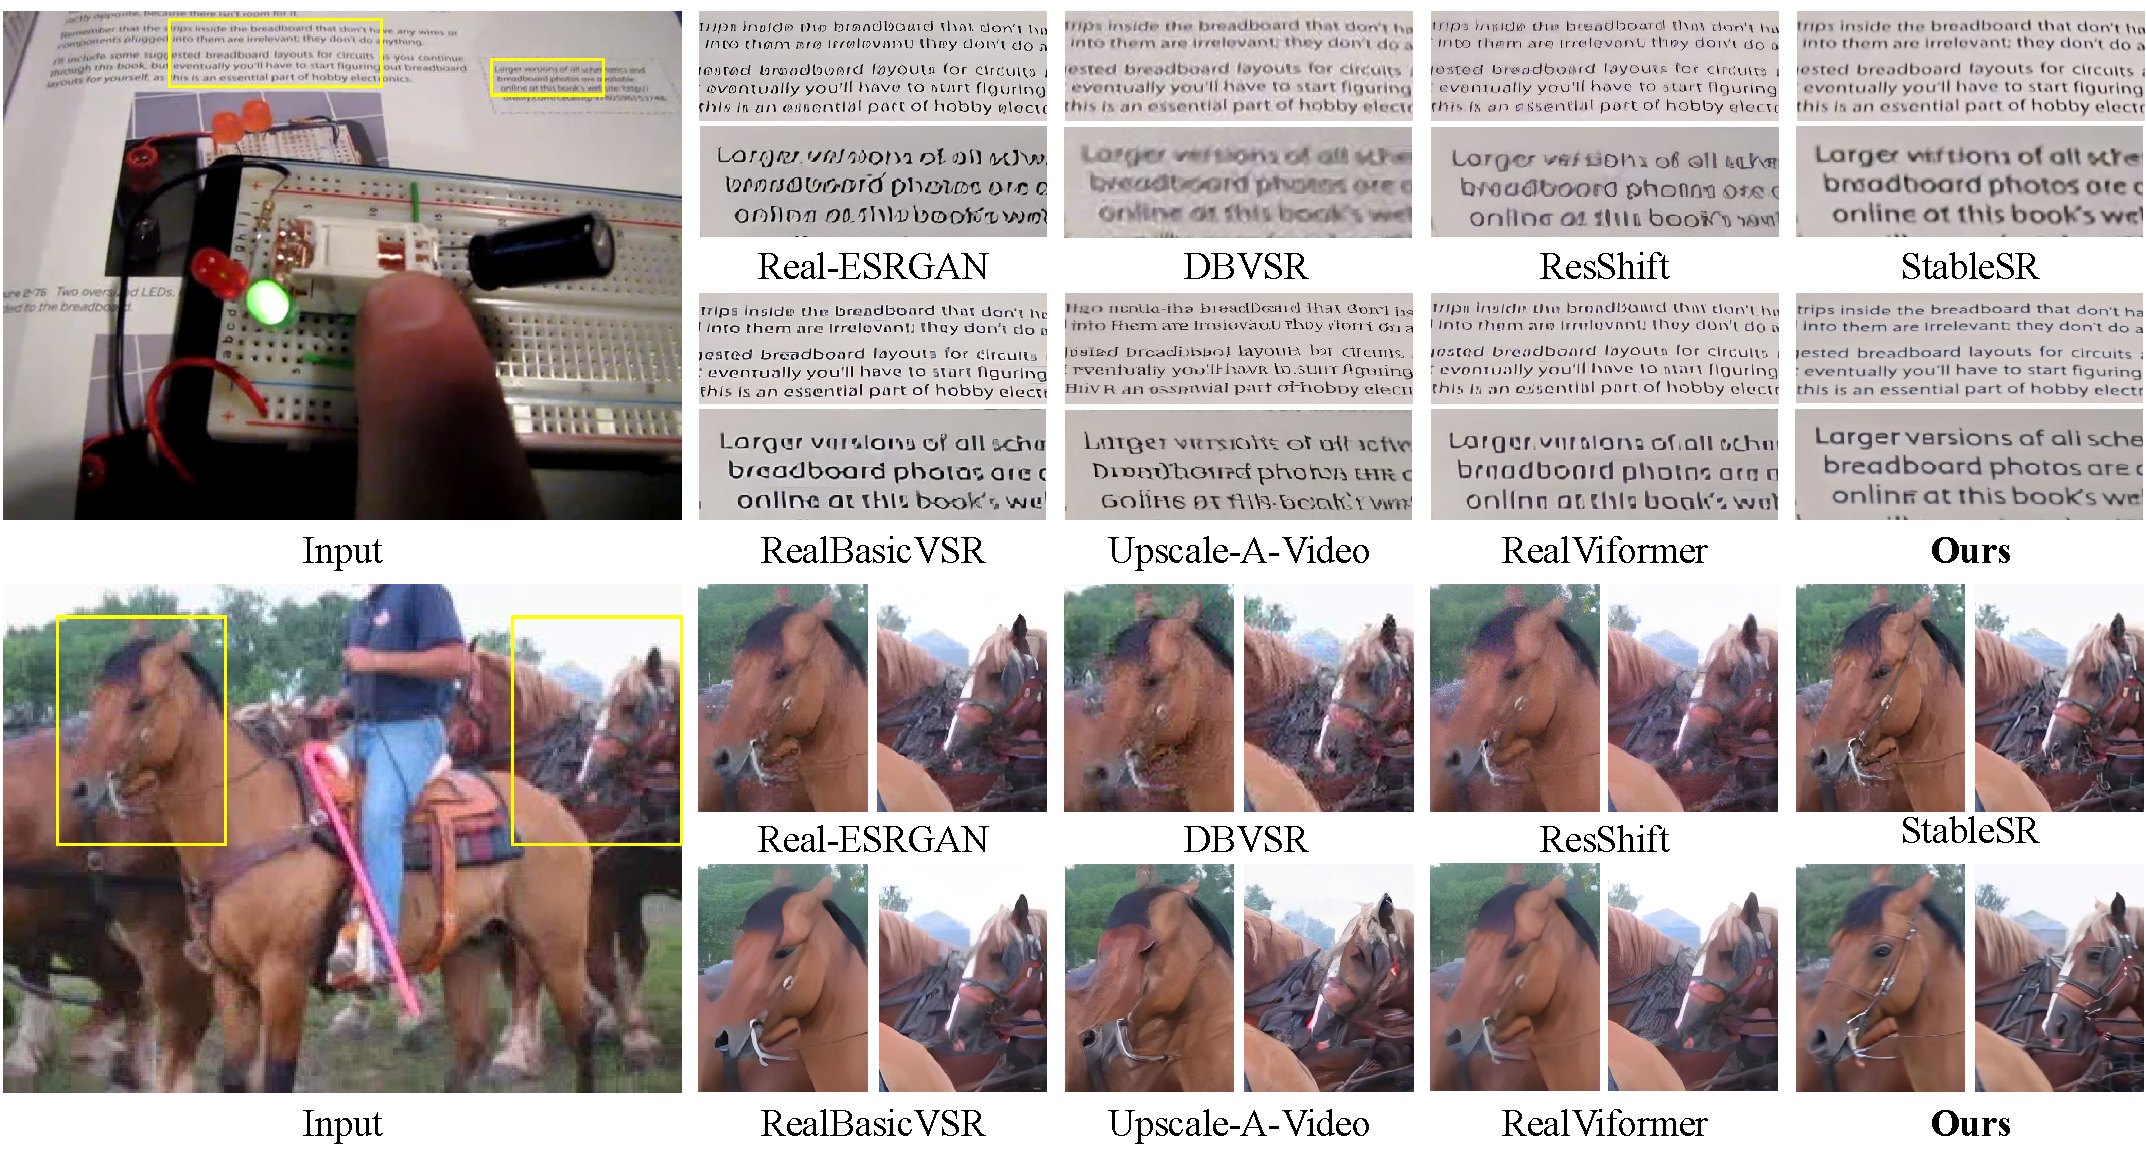
\includegraphics[width=1\linewidth]{figure/qualitive2.pdf}
    \caption{Qualitative comparisons on real-world test videos in VideoLQ \cite{chan2022investigating} dataset. \textbf{(Zoom-in for best view)}}
    \label{fig:qualitive2}
\end{figure*}

\begin{figure*}
    \centering
    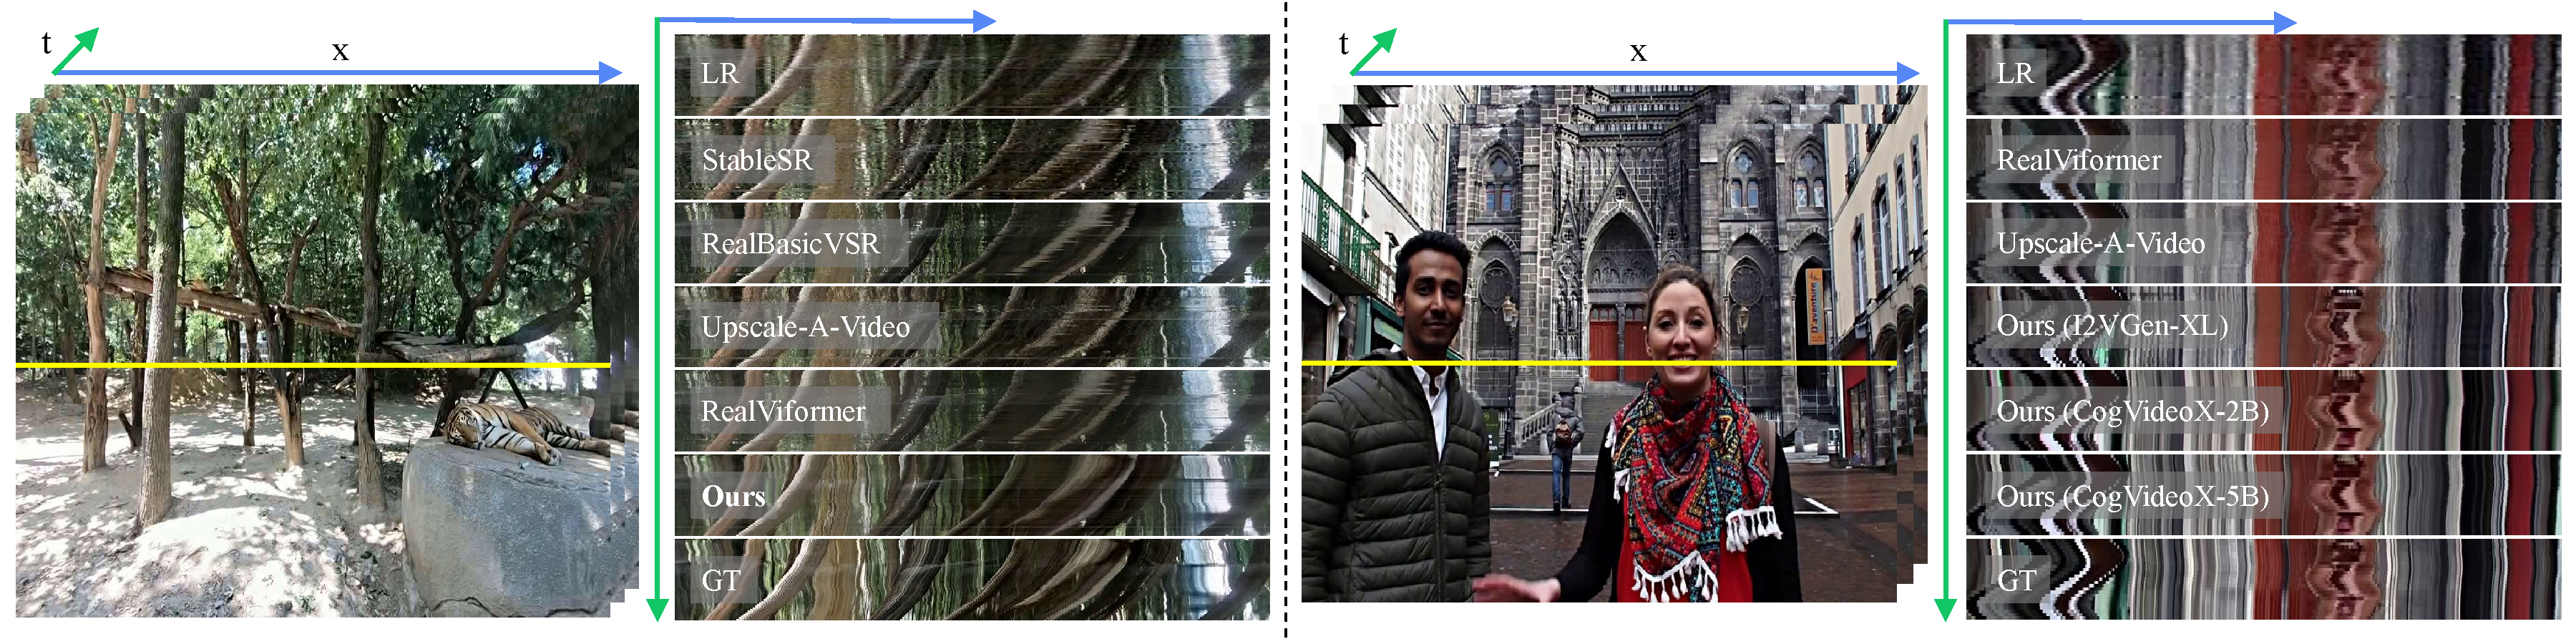
\includegraphics[width=\linewidth]{figure/temporal.pdf}
    \caption{Qualitative comparisons on temporal consistency in REDS30 \cite{nah2019ntire} and OpenVid dataset. \textbf{(Zoom-in for best view)}}
    \label{fig:temp_consis}
\end{figure*}

\subsection{Datasets and Implementation}
\noindent
\textbf{Training Datasets.}
We train~\name~using the subset of OpenVid-1M~\cite{nan2024openvid}, containing $\sim$200K text-video pairs. The OpenVid-1M dataset is a high-quality video dataset consisting of over 1 million in-the-wild video clips with detailed captions, where the minimum resolution is $512$$\times$$512$ and the average length is 7.2 seconds. Utilizing this large-scale high-quality data for training further improves our model's restoration capacity for real-world VSR. More training dataset comparisons can be found in Table \ref{tab:dataset}.
We generate the LR-HR video pairs following the degradation strategy in Real-ESRGAN \cite{wang2021realesrgan}, combined with video compression operations, resulting in severe degradation similar to the approach used in RealBasicVSR \cite{chan2022investigating}.

\begin{table}[]
    \centering
    \caption{Training dataset comparison.}
    \resizebox{1\linewidth}{!}{
    \begin{tabular}{ccccc}
    \hline
       Method & Dataset & Size & $\#$Frames & Resolution \\ \hline
       UAV\cite{zhou2024upscale} & WebVid \cite{bain2021frozen} + YouHQ \cite{zhou2024upscale} & 335K+37K & - & 336$\times$596, 1080$\times$1920 \\
       RealViformer\cite{zhang2024realviformer} & REDS \cite{nah2019ntire} & 300K & 100 & 720$\times$1280 \\
       Ours & OpenVid \cite{nan2024openvid} & 200K & 32 & 720$\times$1280 \\ \hline
    \end{tabular}
    }
    \label{tab:dataset}
\end{table}


\noindent
\textbf{Testing Datasets.}
We evaluate our method on both synthetic and real-world datasets. 
As for synthetic testing datasets, we follow the same degradation pipeline in training to generate LR videos from HR ones to construct three synthetic datasets (\textit{i.e.}, UDM10 \cite{yi2019progressive}, REDS30 \cite{nah2019ntire}, and OpenVid30). The OpenVid30 is split from OpenVid-1M \cite{nan2024openvid} ensuring no overlap with the training dataset and comprises the first approximately 100 frames of 30 videos. For the real-world dataset, we choose VideoLQ \cite{chan2022investigating} which contains 50 videos, each with 100 frames.


\noindent
\textbf{Training Details.}
%We take I2VGen-XL \cite{zhang2023i2vgen} as the T2V backbone by default. 
By default, we adopt I2VGen-XL~\cite{zhang2023i2vgen} as our T2V backbone.
For fast convergence, we initialize the model using the weights from VEnhancer~\cite{he2024venhancer}. We then train the ControlNet and inserted LIEM to adapt the T2V model for the real-world VSR task. Specifically, we train~\name~on $8$ NVIDIA A100-80G GPUs with $15$K iterations and a batch size of $8$. 
The training data is $720$$\times$$1280$ with $32$ frames. We use AdamW \cite{loshchilov2017decoupled} as the optimizer with a learning rate of 5e-5.

\noindent
\textbf{Evaluation Metrics.}
We adopt six metrics to evaluate the VSR outputs from several different perspectives: image fidelity (PSNR), perceptual similarity (SSIM \cite{wang2004image}, LPIPS \cite{zhang2018lpips}), quality (ILNIQE \cite{zhang2015ilniqe}), video clarity (DOVER \cite{wu2023dover}) and temporal consistency ($E^*_{warp}$ \cite{Lai2018warping, liu2024evalcrafter}). 
For synthetic datasets, we calculate PSNR, SSIM and LPIPS between the output and ground-truth frames, along with DOVER and flow warping error (\textit{i.e.}, $E^*_{warp}$) of output videos. For real-world dataset, because of no ground-truth videos, we use three non-reference metrics: ILNIQE, DOVER, and $E^*_{warp}$.
%

\subsection{Comparisons}
To verify the effectiveness of our approach, we compare~\name~with several state-of-the-art methods, including Real-ESRGAN \cite{wang2021realesrgan}, DBVSR \cite{pan2021deep}, RealBasicVSR \cite{chan2022investigating}, RealViformer \cite{zhang2024realviformer}, ResShift \cite{yue2024resshift}, StableSR \cite{wang2024exploiting}, and Upscale-A-Video \cite{zhou2024upscale}.


\noindent
\textbf{Quantitative Evaluation.}
% We first show the quantitative comparison on synthetic and real-world benchmarks. As shown in Table \ref{tab:my_label}, our~\name~achieves the highest DOVER across all four datasets, demonstrating its ability to remove degradation and generate clear details. Moreover, our~\name~achieves the best LPIPS and SSIM scores on UDM10 and OpenVid30, indicating its capability to generate realistic details while maintaining good fidelity. Thanks to the temporal priors in the T2V model, our~\name~generates the best E$^*_{warp}$ on UDM10 and OpenVid30 without combining optical flow map. Although our~\name~does not achieve the best scores on most metrics for REDS30 and VideoLQ, \textit{our visual results are preferred by human evaluators}. Additional evidence is provided in the Qualitative Evaluation and User Study sections (see Appendix).
As shown in Table \ref{tab:my_label}, we calculate five metrics on each synthetic benchmark. Our~\name~achieves the best scores in four out of these five metrics (SSIM, LPIPS, DOVER, and $E^*_{warp}$) on both UDM10 and OpenVid30 datasets, along with the second-best PSNR scores. This indicates that~\name~can generate realistic details with good fidelity and robust temporal consistency.
Moreover, we evaluate three non-reference metrics on a real-world dataset. On this dataset,~\name~achieves the best score in DOVER and the second-best scores in ILNIQE and $E^*_{warp}$. These results demonstrate that~\name~can effectively restore real-world videos with high spatial and temporal quality.
Additionally, our visual results on both real-world and synthetic datasets are preferred by human evaluators, as detailed in the User Study section (see Appendix).

\vspace{-0.3mm}
\noindent
\textbf{Qualitative Evaluation.}
To intuitively demonstrate the effectiveness of the proposed~\name, we present visual results on both synthetic and real-world datasets in Figure \ref{fig:qualitive1} and \ref{fig:qualitive2}, respectively. As shown, our~\name~generates the most realistic spatial details and exhibits the best degradation removal capability. Specifically, the first example in Figure \ref{fig:qualitive2} illustrates that ~\name~reconstructs the text structure most effectively, thanks to the T2V prior efficiently capturing temporal information, and the DF loss that improves the fidelity. Furthermore, the T2V model has a strong spatial prior, which helps generate more realistic details and structures, such as the human hand in Figure \ref{fig:qualitive1} and the horse shape and fur in Figure \ref{fig:qualitive2}.

We also compare the temporal consistency in Figure \ref{fig:temp_consis}. As observed in the left of Figure \ref{fig:temp_consis}, StableSR demonstrates the most temporal inconsistency, primarily because it is originally designed for image super-resolution. Although RealBasicVSR, Upscale-A-Video, and RealViformer incorporate optical flow maps to enhance temporal consistency, they still face challenges in generating consistent results under complex degraded video conditions, as the optical flow maps may not always be accurate. In contrast, our proposed~\name~achieves the best temporal consistency, thanks to the powerful temporal prior inherent in the T2V model, which effectively helps reconstruct temporal information \textit{even without the use of optical flow maps.}


% \noindent
% \textbf{User Study.}


\subsection{Ablation Study}

\begin{figure*}
    \centering
    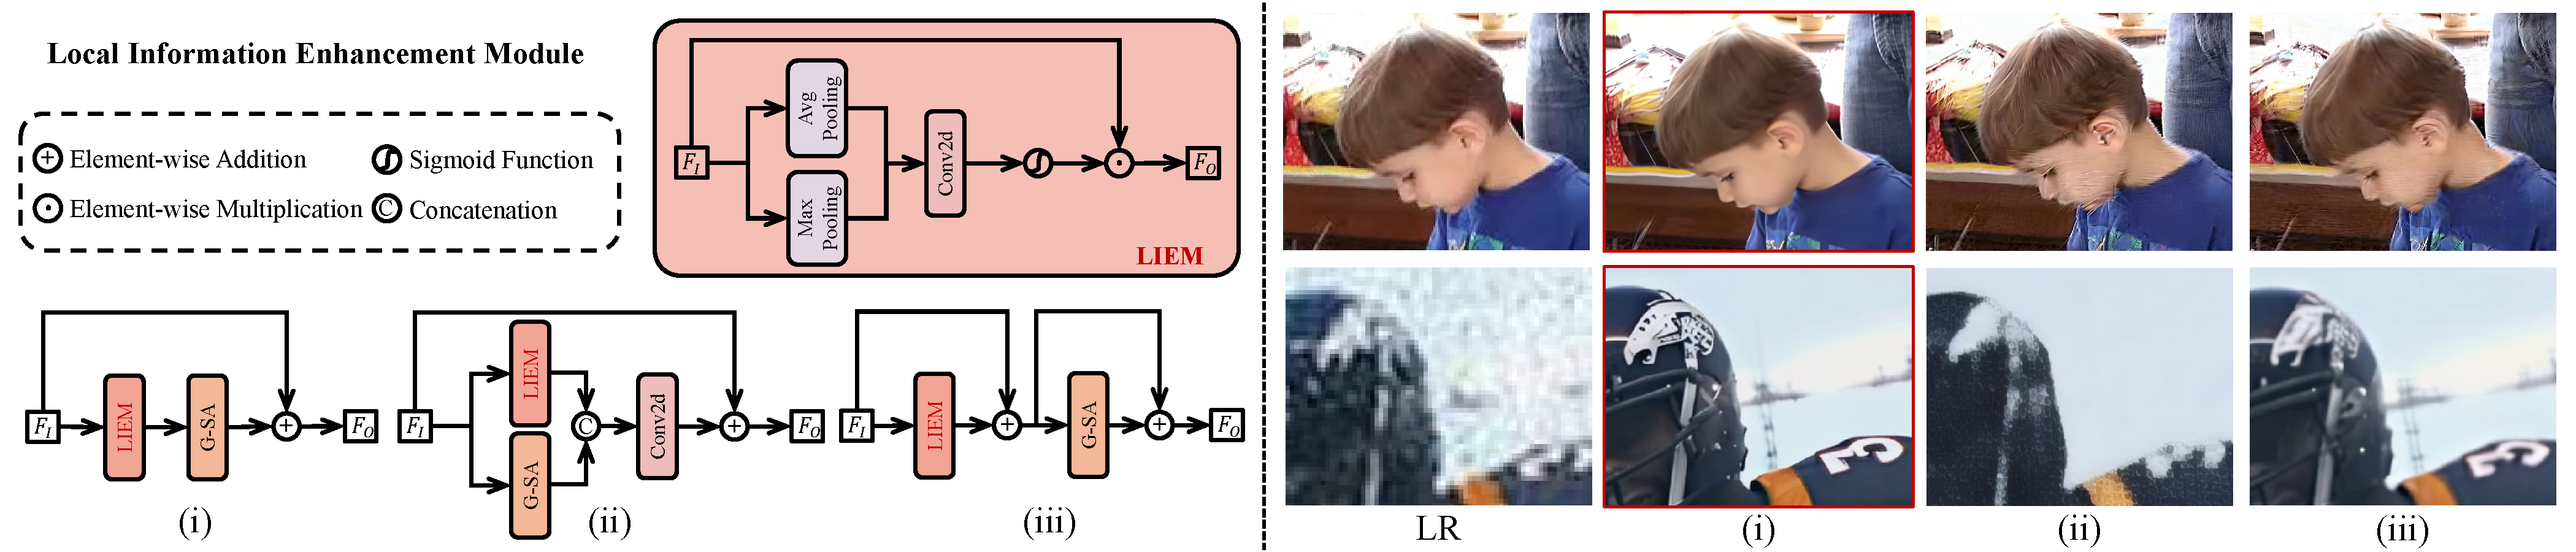
\includegraphics[width=\linewidth]{figure/liem_ablation.pdf}
    \caption{Ablation study about LIEM. \textbf{Left:} illustration of different insertion positions of LIEM and the structure of LIEM. \textbf{Right:} visual comparison on real-world and synthetic videos with different LIEM positions.}
    \label{fig:liem_ablation}
\end{figure*}

\begin{table}[t]
    \centering
    \caption{Ablation of LIEM position.}
    \resizebox{\linewidth}{!}{
    \begin{tabular}{c|cc|ccc}
    \hline
       Position & Spa-Local & Temp-Local & PSNR$\uparrow$ & LPIPS$\downarrow$ & $E_{warp}^*\downarrow$ \\ \hline
        \multirow{4}{*}{(i)} & ~ & ~ & 23.14 & 0.2015 & 2.83 \\
        ~ & $\checkmark$ & ~ & 23.61 & 0.2013 & 2.82 \\
        ~ & ~ & $\checkmark$ & 23.65 & \underline{0.1945} & 2.92 \\ \cline{2-3}
        ~ & \multirow{3}{*}{$\checkmark$} & \multirow{3}{*}{$\checkmark$} & \cellcolor{lightgray}\underline{23.69} & \cellcolor{lightgray}\textbf{0.1943} & \cellcolor{lightgray}\underline{2.74} \\ \cline{1-1}
        (ii) & ~ & ~ & 23.27 & 0.2363 & 3.57 \\
        (iii) & ~ & ~ & \textbf{24.51} & 0.2094 & \textbf{1.99} \\ \hline
    \end{tabular}}
    \label{tab:position_ablation}
\end{table}

\noindent
\textbf{Local Information Enhancement Module.}
\label{sec:liem_ablation}
We primarily investigate the impact of introducing LIEM in different ways. First, we find that adding LIEM on both spatial and temporal blocks achieves the best results as shown in Table \ref{tab:position_ablation}. Second, we consider three connection types as shown in Figure \ref{fig:liem_ablation} (Left). From visual results in Figure \ref{fig:liem_ablation} (Right) and quantitative results in Table \ref{tab:position_ablation}, we find that position (i) achieves the best results. This phenomenon can be attributed to the fact that, with most weights frozen to preserve the prior, the newly added blocks can influence the model's mapping process. However, the impact at positions (ii) and (iii) is too large, making it difficult for the model to fine-tune and adapt to this change, resulting in poor performance.

\begin{table}[t]
    \centering
    \caption{Ablation of different variants of DF loss.}
    \begin{tabular}{cc|ccc}
    \hline
       Seperate & Type & PSNR$\uparrow$ & LPIPS$\downarrow$ & $E_{warp}^*\downarrow$ \\ \hline
       \multicolumn{2}{c|}{w/o Frequency Loss} & 23.69 & 0.1943 & 2.74 \\ \hline
        - & - & \underline{23.72} & \underline{0.1941} & \underline{2.71} \\
        $\checkmark$ & Inverse & 23.67 & 0.1945 & 2.83 \\
        $\checkmark$ & Direct & \cellcolor{lightgray}\textbf{23.85} & \cellcolor{lightgray}\textbf{0.1903} & \cellcolor{lightgray}\textbf{2.69} \\ \hline
    \end{tabular}
    \label{tab:daf_ablation1}
\end{table}

\begin{table}[t]
    \centering
    \caption{Ablation of $b(t)$ and $\alpha$ in $c(t)$.}
    \begin{tabular}{c|c|ccc}
    \hline
       b(t) & $\alpha$ & PSNR$\uparrow$ & LPIPS$\downarrow$ & $E_{warp}^*\downarrow$ \\ \hline
       \multirow{5}{*}{Linear} & 0.25 & 23.76 & 0.2030 & 2.72 \\
        ~ & 0.5 & 23.71 & 0.2010 & 2.75 \\
        ~ & 1 & \underline{23.85} & \underline{0.1903} & \underline{2.69} \\
        ~ & 1.5 & 23.53 & 0.1928 & 2.81 \\ \cline{2-2}
        ~ & \multirow{2}{*}{2} & \cellcolor{lightgray}\textbf{23.91} & \cellcolor{lightgray}\textbf{0.1885} & \cellcolor{lightgray}\textbf{2.61} \\ \cline{1-1}
        Exponential & ~ & 23.68 & 0.1990 & 2.78 \\
        \hline
    \end{tabular}
    \label{tab:daf_ablation2}
\end{table}

% \begin{table}[t]
%     \centering
%     \caption{Ablation of DAF Loss.}
%     \begin{tabular}{ccc|ccc}
%     \hline
%        Method & $X_H$ & t & PSNR$\uparrow$ & LPIPS$\downarrow$ & $E_{warp}^*\downarrow$ \\ \hline
%        w/o adaptation & \multicolumn{2}{c|}{-} & ~ & ~ & ~ \\ \hline
%        \multirow{3}{*}{w adaptation} & $\checkmark$ & ~ & ~ & ~ & ~ \\
%        ~ & $\checkmark$ & ~ & ~ & ~ & ~ \\
%        ~ & $\checkmark$ & ~ & ~ & ~ & ~ \\ \hline
%     \end{tabular}
%     \label{tab:daf_ablation3}
% \end{table}

% \begin{figure}
%     \centering
%     \includegraphics[width=1\linewidth]{figure/cutoff_timestep.png}
%     \caption{Learned Cutoff Curves.}
%     \label{fig:cutoff_timestep}
% \end{figure}

\begin{figure}
    \centering
    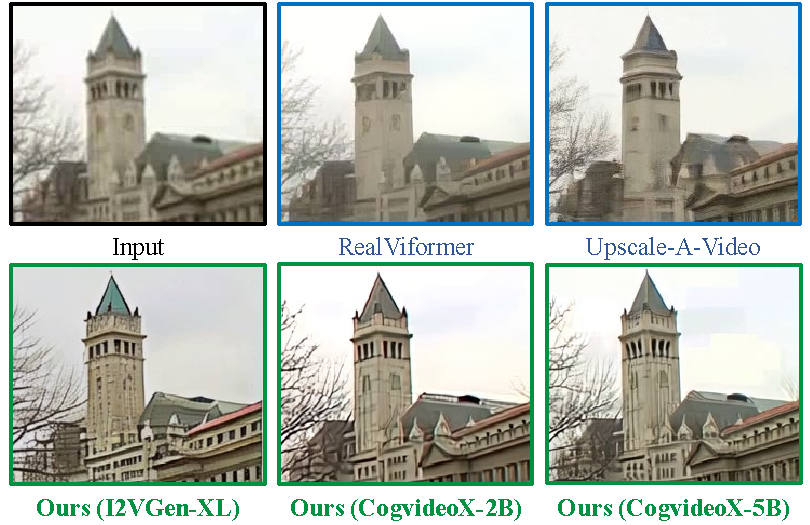
\includegraphics[width=1\linewidth]{figure/t2v_ablation.pdf}
    \caption{Illustration on scaling up with larger t2v models on a real-world low-quality video. \textbf{(Zoom-in for best view)}}
    \label{fig:ablation3}
\end{figure}

\noindent
\textbf{Dynamic Frequency Loss.}
\label{ablation:daf}
First, we investigate the impact of different variants of frequency loss. As shown in Table~\ref{tab:daf_ablation1}, ``Separate" indicates whether the frequency components are separated into high and low frequency, constraining them individually. 
``Type" refers to the specific definition of the DF loss: if set to ``inverse," a higher weight is given to high frequencies in the early stages and a lower weight to low frequencies; if set to ``direct", a higher weight is given to low frequencies initially and a lower weight to high frequencies, which is matching the analysis in Sec.~\ref{subsec:daf}. As observed, separating the frequency components and prioritizing low-frequency reconstruction early on yield the best perceptual quality while maintaining high fidelity. Second, we explore the optimal settings for $b(t)$ and $\alpha$ in $c(t)$. As shown in Table~\ref{tab:daf_ablation2}, using a linear form for $b(t)$ with $\alpha=2$ for $c(t)$ yields the best results. Therefore, we adopt this DF loss configuration for training our model and comparing it with other state-of-the-art methods.

% Finally, we introduce the adaptive filter and demonstrate its effect. As shown in Table \ref{tab:daf_ablation3}, . Moreover, we show the learned adaptive filter value across different diffusion steps in Figure \ref{fig:cutoff_timestep}.


\begin{table}[t]
    \centering
    \caption{Effectiveness of T2V diffusion prior for real-world VSR.}
    \resizebox{\linewidth}{!}{
    \begin{tabular}{c|cc|ccc}
    \hline
       \multirow{2}{*}{Metrics} & \multirow{2}{*}{UAV} & \multirow{2}{*}{RealViformer} & \multicolumn{3}{c}{Ours} \\
       ~ & ~ & ~ & I2VGen-XL & CogX-2B & CogX-5B \\ \hline
        PSNR$\uparrow$ & 22.46& 22.90& 21.46& \underline{23.18}& \textbf{23.60}\\
        SSIM$\uparrow$ & 0.6552& 0.6944& 0.6715& \underline{0.7112}& \textbf{0.7400}\\
        LPIPS$\downarrow$ & 0.2035& 0.1823& 0.1779& \underline{0.1571}& \textbf{0.1314}\\
        DOVER$\uparrow$ & 0.6609& 0.4286& \underline{0.7267}& 0.6955& \textbf{0.7350}\\
        $E_{warp}^*\downarrow$ & 5.424& 4.75& 5.529& \textbf{3.68} & \underline{4.56}\\ \hline
    \end{tabular}}
    \label{tab:t2v prior}
\end{table}
\vspace{-1mm}



\noindent
\textbf{Scaling up with Larger T2V Models.}
To further validate the effectiveness of T2V diffusion priors for real-world VSR, we replace I2VGen-XL with larger 
%we apply our baseline settings (w/o LIEM and w/o DF Loss) to 
DiT-based \cite{peebles2023scalable} T2V models (\textit{i.e.,} CogVideoX~\cite{cogvideox5b,yang2024cogvideox}), and evaluate results both quantitatively and qualitatively. 
%Since CogVideoX only supports inputs at 480$\times$720 resolution, we create a new test set by cropping 10 videos from OpenVid-1M to this size. As shown in Table \ref{tab:t2v prior}, the powerful T2V models achieve best scores across all metrics, even without task-specific designs. 
Since CogVideoX only supports inputs at 480$\times$720 resolution, we created a new test set by cropping 10 videos from OpenVid-1M \cite{nan2024openvid} to this size. 
As shown in Table~\ref{tab:t2v prior}, the powerful CogVideoX models yield consistent improvements across all metrics. %even without task-specific adaptations.
%
%Additionally, the strong spatio-temporal priors in T2V models allow the restored human face to retain realistic details and natural facial details and clear building structure (see Figure~\ref{fig:ablation3}) while maintaining high temporal consistency (see Figure~\ref{fig:temp_consis} Left). We believe that robust T2V models can serve as a strong base model for video super-resolution tasks.
%
Notably, SSIM improves from 0.6944 to 0.7400, and DOVER increases from 0.6609 to 0.7350, marking a substantial enhancement in visual quality. 
The robust spatio-temporal priors in CogVideoX enable realistic details and clear building structures (Figure~\ref{fig:ablation3}), while maintaining high temporal consistency (Figure~\ref{fig:temp_consis} Right).
Inspired by scaling law \cite{henighan2020scaling, kaplan2020scaling} and our findings, we believe larger, more powerful T2V models will further advance VSR tasks.


% We conduct our evaluation on PSNR, SSIM, LPIPS, DOVER, and $E^*_{warp}$ metrics. We compare with several state-of-the-art VSR methods (\textit{i.e.}, RealBasicVSR \cite{chan2022investigating}, RealViformer \cite{zhang2024realviformer}, and Upscale-A-Video \cite{zhou2024upscale}).
% As shown in Table \ref{tab:t2v prior}, our method with CogVideoX-2B \cite{cogvideox2b} 
% To show the excellent generalization and super-resolution ability of our method on CogVideoX-2B, we present visual results on the specific dataset in Figure \ref{fig:ablation3}. 
